\section{5.3 Control system design}
\subsection{A, Design of a PD controller}
A PD controller is given by the equation $H_{pd}(s) = K_{pd} \frac{1+T_ds}{1+T_fs}$. Using the transfer function \cref{eq:Transfer_function} from $\delta$ to $\psi$ without disturbances we define the open loop system as $H(s) \cdot H_{pd}(s)$. We chose $T_d=T$ to cancel the transfer function time constant. This reduces the order of the transfer function because the two terms cancels out. The open loop transfer function then becomes
\begin{align} \label{eq:transfer_function_open_loop}
    H(s) = \frac{K_{pd}K}{s(1+T_f s)}
\end{align} 
We wish to chose $K_{pd}$ such that the open loop system has $\omega_c = 0.10$ rad/s and a phase margin of $50 \deg$. 
\begin{align}
    \left| H(j\omega_c) \right| = 0 dB = 1 \notag \\
    \left| \frac{K_{pd}K}{j\omega_c(1+T_f j\omega_c)}\right| = 1 \notag \\
    \frac{K_{pd}K}{\omega_c \sqrt{1+T_f^2\omega_c^2}} = 1 \label{eq:length_tf}
\end{align}
The phase margin $\phi$ is defined as 
\begin{align}
    \phi = \angle H(j\omega_c) - (-180^\circ)
\end{align}
and by setting $\phi$ equal to $50^\circ$ we get
\begin{align}
    50^\circ = -90^\circ - \textrm{arctan}(T_f \omega_c)\notag \\
    T_f = \frac{\textrm{tan}(50^\circ-180^\circ+90^\circ}{\omega_c} = 8.4s
\end{align}
Now by inserting the obtained $T_f$ into \cref{eq:length_tf} we can solve for $K_{pd}$.
\begin{align}
    K_{pd} = \frac{\omega_c \sqrt{1+T_f^2\omega_c^2}}{K} = 0.839
\end{align}
\subsection{B, Implementation of PD controller and simulation without disturbances}
We implement the PD controller in Simulink as seen in \cref{fig:simulink_PD} and \cref{fig:simulink_total}. We set the reference $\psi_r = 30$ and simulate the system with only measurement noise, no disturbances. As we can see in \cref{fig:p3pb_rudder_heading} the ship reaches the reference pretty quickly and is able to hold keep the course stable. Thus the autopilot does its job quite satisfyingly. The rudder input is high in the start but as the system stabilizes it the size of the rudder input input moves to zero. It does however have some small vibrations due to the controller being sensitive to the measurement noise. The ship dynamics has a quite negative phase which results in either a slow controller or an oscillating response due to a small phase margin. A PD-controller lifts the phase of the full system and allows for higher $\omega_c$ resulting in quicker and more robust response than a P-controller. 
\begin{figure}
    \centering
    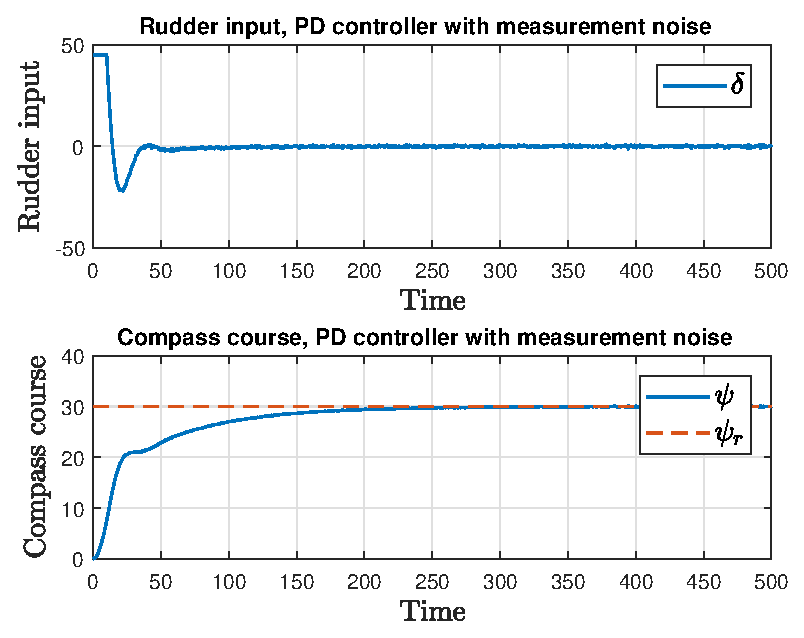
\includegraphics[width = 1.00\textwidth]{figures/plots/P5p3b_rudder_heading.eps}
    \caption{Rudder input and compass course response with a PD controller.}
    \label{fig:p3pb_rudder_heading}
\end{figure}
\subsection{C, Simulation with a current disturbance}
Now we simulate the system with current disturbance, measurement noise but no wave disturbance. As we can see in the \cref{fig:p3pc_rudder_heading}, the autopilot is no longer able to reach the reference of 30$\deg$. A stationary deviation of about 3.5$\deg$ is present. This is expected as we have no integral effect and the PD controller will only change the rudder input if the error changes. The rudder input never reaches zero but constantly tries to counteract the current disturbance.
\begin{figure}
    \centering
    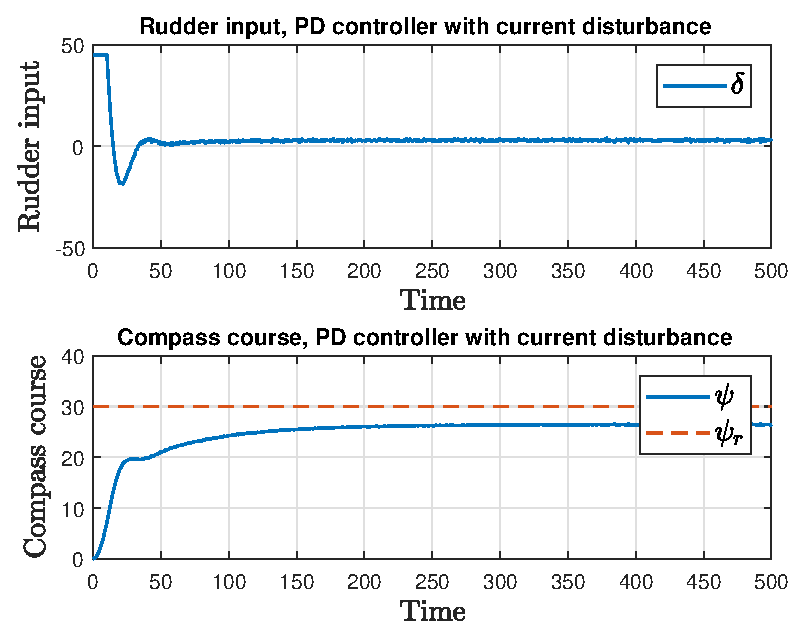
\includegraphics[width = 1.00\textwidth]{figures/plots/P5p3c_rudder_heading.eps}
    \caption{Rudder input and compass course response with a PD controller. Simulated with current disturbance.}
    \label{fig:p3pc_rudder_heading}
\end{figure}
\subsection{D, Simulation with a wave disturbance}
When simulating without current disturbance but with wave disturbance the system reaches the reference of 30$\deg$. With the wave disturbance the signal has a lot of high frequency oscillations as we can see in \cref{fig:p3pd_rudder_heading}. This is due to the high frequency nature of the waves that affect the system. \\
The oscillations are quite small compared to the state and the reference. Therefore it will not affect the system too much. Moreover the noise has a mean of zero, so it will not affect the path of the ship in the long run. The actuation of the rudder is quite oscillatory. This is not ideal and would cause wear on the physical system. Later we will look at how a Kalman filter reduces the use of actuation.  
\begin{figure}
    \centering
    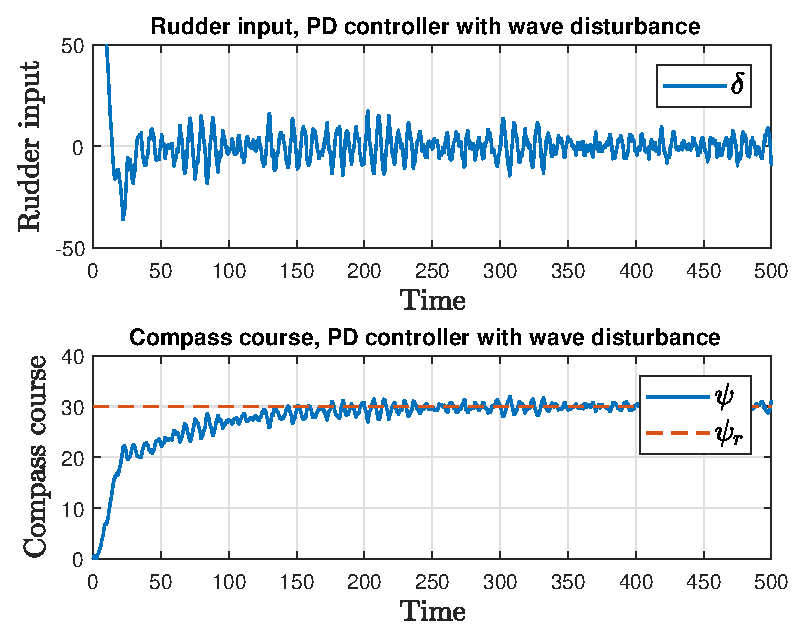
\includegraphics[width = 1.00\textwidth]{figures/plots/P5p3d_rudder_heading.eps}
    \caption{Rudder input and compass course response with a PD controller. Simlutated with wave disturbance.}
    \label{fig:p3pd_rudder_heading}
\end{figure}
